\documentclass{beamer}
\usepackage[utf8]{inputenc}

\usetheme{Madrid}
\usecolortheme{default}
\usepackage{amsmath,amssymb,amsfonts,amsthm}
\usepackage{txfonts}
\usepackage{tkz-euclide}
\usepackage{listings}
\usepackage{adjustbox}
\usepackage{array}
\usepackage{tabularx}
\usepackage{gvv}
\usepackage{lmodern}
\usepackage{circuitikz}
\usepackage{tikz}
\usepackage{graphicx}
\usepackage{amsmath}

\setbeamertemplate{page number in head/foot}[totalframenumber]

\usepackage{tcolorbox}
\tcbuselibrary{minted,breakable,xparse,skins}



\definecolor{bg}{gray}{0.95}
\DeclareTCBListing{mintedbox}{O{}m!O{}}{%
  breakable=true,
  listing engine=minted,
  listing only,
  minted language=#2,
  minted style=default,
  minted options={%
    linenos,
    gobble=0,
    breaklines=true,
    breakafter=,,
    fontsize=\small,
    numbersep=8pt,
    #1},
  boxsep=0pt,
  left skip=0pt,
  right skip=0pt,
  left=25pt,
  right=0pt,
  top=3pt,
  bottom=3pt,
  arc=5pt,
  leftrule=0pt,
  rightrule=0pt,
  bottomrule=2pt,
  toprule=2pt,
  colback=bg,
  colframe=orange!70,
  enhanced,
  overlay={%
    \begin{tcbclipinterior}
    \fill[orange!20!white] (frame.south west) rectangle ([xshift=20pt]frame.north west);
    \end{tcbclipinterior}},
  #3,
}
\lstset{
    language=C,
    basicstyle=\ttfamily\small,
    keywordstyle=\color{blue},
    stringstyle=\color{orange},
    commentstyle=\color{green!60!black},
    numbers=left,
    numberstyle=\tiny\color{gray},
    breaklines=true,
    showstringspaces=false,
}


\title 
{4.12.26}
\date{September 24,2025}


\author 
{Abhiram Reddy-AI25BTECH11021}



\begin{document}


\frame{\titlepage}

% --- FRAME 1: Question ---
\begin{frame}{Question}
    \framesubtitle{Locus of the Foot of the Perpendicular}
    
    The line $\frac{x}{a} + \frac{y}{b} = 1$ moves in such a way that the condition
    $$\frac{1}{a^2} + \frac{1}{b^2} = \frac{1}{c^2}$$
    is satisfied, where $c$ is a constant.
    
    Prove that the locus of the foot of the perpendicular from the origin on the given line is $x^2 + y^2 = c^2$, using vector algebra with matrix notation and transpose.
\end{frame}

% --- FRAME 2: Step 1 & 2 ---
\begin{frame}{Step 1: Vector Representation}
    \framesubtitle{Vector and Perpendicularity Conditions}
    
    \begin{enumerate}
        \item \textbf{Line Equation:} The line $L$ is $\frac{x}{a} + \frac{y}{b} = 1$.
        $$L: \mathbf{r}^T \mathbf{n} = 1, \quad \text{where } \mathbf{r} = \begin{pmatrix} x \\ y \end{pmatrix}, \mathbf{n} = \begin{pmatrix} 1/a \\ 1/b \end{pmatrix} \quad \text{(Equation 1)}$$
        
        \item \textbf{Foot of Perpendicular $P$:} Let $P(x_0, y_0)$ have position vector $\mathbf{p} = \begin{pmatrix} x_0 \\ y_0 \end{pmatrix}$.
        
        \item \textbf{Perpendicularity $\mathbf{p} \parallel \mathbf{n}$:} The vector $\mathbf{p}$ is parallel to the normal $\mathbf{n}$.
        $$\mathbf{p} = \lambda \mathbf{n} \quad \text{for some scalar } \lambda \quad \text{(Equation 2)}$$
        This gives the component relations:
        $$\frac{1}{a} = \frac{x_0}{\lambda} \quad \text{and} \quad \frac{1}{b} = \frac{y_0}{\lambda} \quad \text{(Equation 3)}$$
    \end{enumerate}
\end{frame}

% --- FRAME 3: Step 3 & 4 ---
\begin{frame}{Steps 3 \& 4: Locus Derivation}
    \framesubtitle{Substituting into the Line and Constraint Equations}
    
    \begin{enumerate}
        \setcounter{enumi}{3}
        \item \textbf{$P$ lies on $L$:} Substitute $\mathbf{p}$ into the line equation (Eq. 1):
        $$\mathbf{p}^T \mathbf{n} = 1 \implies \frac{x_0}{a} + \frac{y_0}{b} = 1$$
        Substitute (Eq. 3) into the above:
        $$\frac{x_0^2}{\lambda} + \frac{y_0^2}{\lambda} = 1 \implies x_0^2 + y_0^2 = \lambda \quad \text{(Equation 4)}$$
        In matrix form: $\mathbf{p}^T \mathbf{p} = \lambda$.
        
        \item \textbf{Apply the Constraint:} Substitute (Eq. 3) into the given condition $\frac{1}{a^2} + \frac{1}{b^2} = \frac{1}{c^2}$:
        $$\left(\frac{x_0}{\lambda}\right)^2 + \left(\frac{y_0}{\lambda}\right)^2 = \frac{1}{c^2}$$
        $$\frac{x_0^2 + y_0^2}{\lambda^2} = \frac{1}{c^2} \quad \text{(Equation 5)}$$
        
        \item \textbf{Solve for Locus:} Substitute $\lambda$ from (Eq. 4) into (Eq. 5):
        $$\frac{\lambda}{\lambda^2} = \frac{1}{c^2} \implies \frac{1}{\lambda} = \frac{1}{c^2} \implies \lambda = c^2 \quad \text{(Equation 6)}$$
        
        \item \textbf{Final Locus:} Substitute $\lambda = c^2$ back into (Eq. 4):
        $$x_0^2 + y_0^2 = c^2$$
        The locus of $P(x_0, y_0)$ is:
        $$x^2 + y^2 = c^2 \quad \text{(Equation 7)}$$
    \end{enumerate}
\end{frame}

% --- FRAME 4: C Code - Part 1 (Function) ---
\begin{frame}[fragile]{C Code: Locus Verification Function}
    \framesubtitle{Main Formula: $x^2 + y^2 = c^2$}
    
    The main formula is the equation of the locus. The C function verifies if a given point $(x, y)$ lies on this locus for a constant $c$.
    
    \lstset{style=CStyle}
    \begin{lstlisting}[language=C]
#include <stdio.h>
#include <math.h>

int verify_locus(double x, double y, double c) {
    double lhs = (x * x) + (y * y);
    double rhs = c * c;
    double tolerance = 1e-9; 
    
    if (fabs(lhs - rhs) < tolerance) {
        return 1;
    } else {
        return 0;
    }
}
    \end{lstlisting}
\end{frame}

% --- FRAME 5: C Code - Part 2 (Main) ---
\begin{frame}[fragile]{C Code: Main Execution}
    \framesubtitle{Testing the Locus Formula}
    
    \lstset{style=CStyle}
    \begin{lstlisting}[language=C, firstnumber=14]
int main() {
    double constant_c = 5.0; // Locus is x^2 + y^2 = 25

    double x1 = 3.0; // Point (3, 4) is on the locus
    double y1 = 4.0;
    
    if (verify_locus(x1, y1, constant_c)) {
        printf("Point (%.2f, %.2f) IS on the locus x^2 + y^2 = %.2f\n", 
               x1, y1, constant_c * constant_c);
    } else {
        printf("Point (%.2f, %.2f) is NOT on the locus.\n", x1, y1);
    }

    double x2 = 1.0; // Point (1, 1) is not on the locus
    double y2 = 1.0;

    if (verify_locus(x2, y2, constant_c)) {
        printf("Point (%.2f, %.2f) IS on the locus x^2 + y^2 = %.2f\n", 
               x2, y2, constant_c * constant_c);
    } else {
        printf("Point (%.2f, %.2f) is NOT on the locus x^2 + y^2 = %.2f\n", 
               x2, y2, constant_c * constant_c);
    }

    return 0;
}
    \end{lstlisting}
\end{frame}

% --- FRAME 6: Python Code - Part 1 (Setup) ---
\begin{frame}[fragile]{Python Code: Setup and Locus Data}
    \framesubtitle{Generating Data for the Plot}
    
    We use $c=5$ and an example line with intercepts $a=25/3$ and $b=25/4$.
    
    \lstset{style=PythonStyle}
    \begin{lstlisting}[language=Python]
import numpy as np
import matplotlib.pyplot as plt

# 1. Define the constant c and the locus (x^2 + y^2 = c^2)
c = 5.0
c_squared = c * c

# Generate points for the circle (Locus)
theta = np.linspace(0, 2 * np.pi, 100)
x_locus = c * np.cos(theta)
y_locus = c * np.sin(theta)

# 2. Define a specific variable line and its foot of the perpendicular P(x0, y0)
x0 = 3.0
y0 = 4.0

# Intercepts: a = c^2/x0 and b = c^2/y0
a = 25.0 / x0
b = 25.0 / y0

# Generate points for the variable line L
x_line = np.linspace(0, a, 100)
y_line = (c_squared - x_line * x0) / y0
    \end{lstlisting}
\end{frame}

% --- FRAME 7: Python Code - Part 2 (Plotting) ---
\begin{frame}[fragile]{Python Code: Plotting the Graphs}
    \framesubtitle{Visualization of the Locus and an Example Line}
    
    \lstset{style=PythonStyle}
    \begin{lstlisting}[language=Python]
# 3. Create the plot
plt.figure(figsize=(8, 8))

# Plot the Locus (Circle)
plt.plot(x_locus, y_locus, 'r--', label=f'Locus: $x^2 + y^2 = {c_squared:.0f}$')

# Plot the Variable Line L
plt.plot(x_line, y_line, 'b-', label=f'Variable Line L: $\\frac{{x}}{{{a:.2f}}} + \\frac{{y}}{{{b:.2f}}} = 1$')

# Plot the Foot of the Perpendicular P and Origin O
plt.plot(x0, y0, 'go', markersize=8, label=f'Foot P({x0:.0f}, {y0:.0f})')
plt.plot([0, x0], [0, y0], 'g-', linestyle=':', linewidth=2, label='Perpendicular Segment $\\mathbf{OP}$')
plt.plot(0, 0, 'kx', markersize=8, label='Origin O(0, 0)')

# Set limits and aspect ratio
plt.xlim(-c - 2, c + 2)
plt.ylim(-c - 2, c + 2)
plt.gca().set_aspect('equal', adjustable='box')

# Add labels and legend
plt.xlabel('$x$')
plt.ylabel('$y$')
plt.title('Locus of the Foot of the Perpendicular')
plt.grid(True)
plt.legend(loc='lower left')

# Note: In a live environment, plt.show() would display the plot.
# For Beamer, we just show the code.
# plt.show() 
    \end{lstlisting}
\end{frame}

\begin{frame}{Plot}
    \centering
    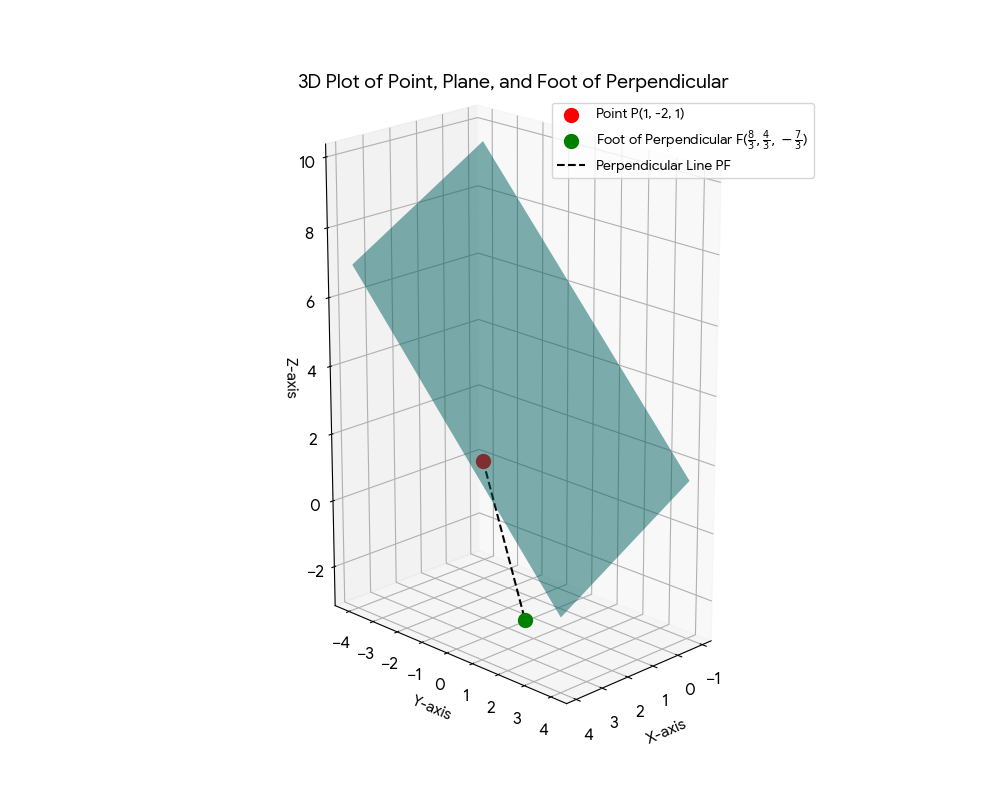
\includegraphics[width=\columnwidth, height=0.8\textheight, keepaspectratio]{figs/python_plot.png}     
\end{frame}


\end{document}